\textbf{SLOW BLUES in G : Backing Track}\\
Practice lesson 4 along to this: \\ 
https://www.youtube.com/watch?v=fmxIvei04Xg\\



    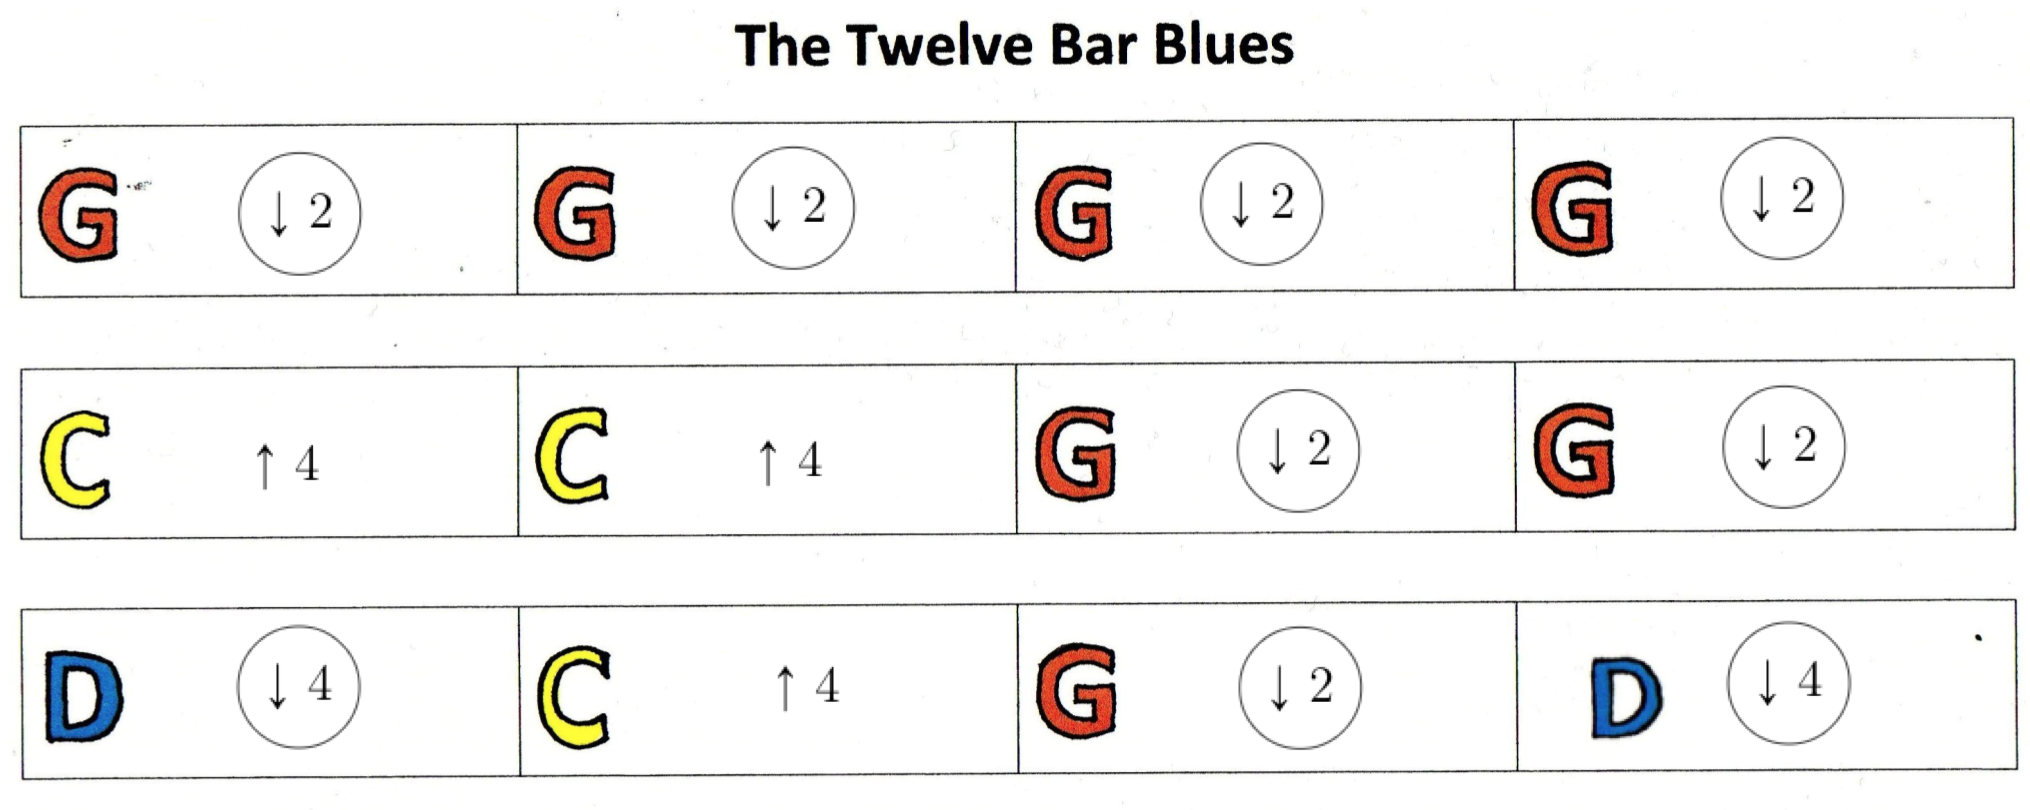
\includegraphics[scale=0.4]{12barbluesharmonica}
    
    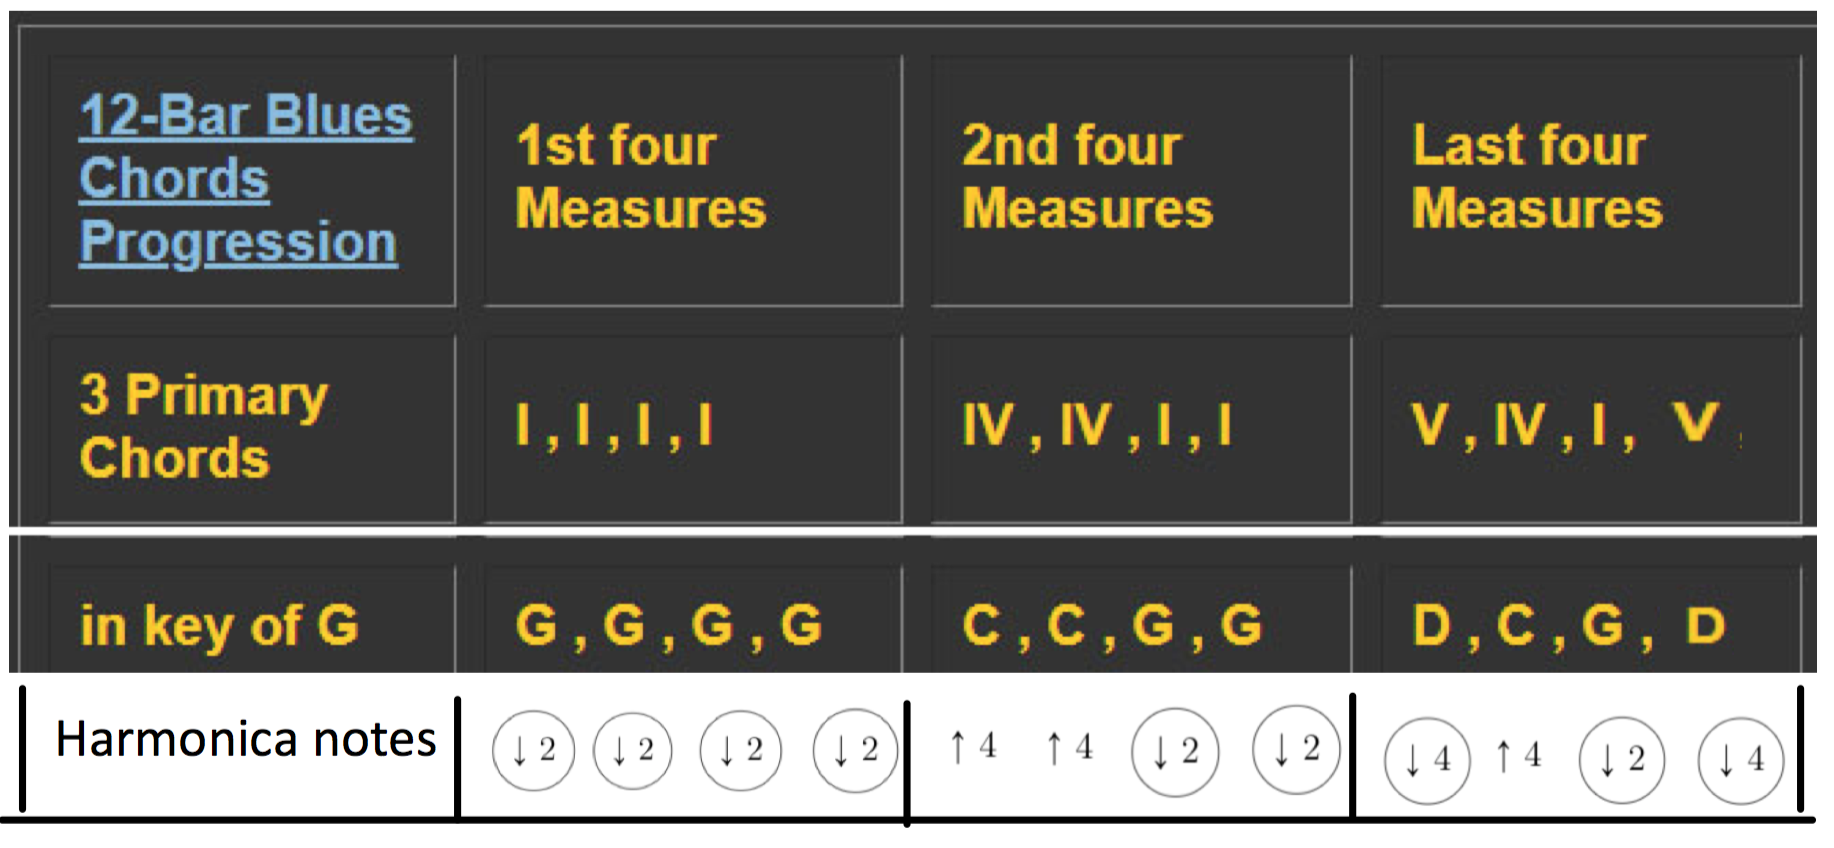
\includegraphics[scale=0.4]{12barbluesharmonica2}

\newpage

\section{Riff 7 to drill this week- a riff to practice playing quietly and clearly}        
% \2\3\4 
\4\3\2

\section{Riff 7.1}
\4\3\2\3\2 \\
\textbf{Some different ways to play this:} \\
% \bi
- All notes connected (one stream of air) \\
- All notes individually\\
\textbf{- All notes tongued (Normal - full duration of the note held}\\
- All notes tongued (Stoccato - very short notes)
% \ei

\subsection{new riff 8}
\e\4 \4 \\ 
\4\e\3\2 \\

\subsection{new riff 8.1 - first note tongued}

\fdbta  \nearrow$ \4 \fdta \\
\fdbta  \nearrow$ \4 \fdta \\
\fdbta  \nearrow$ \4 \fdta \\
\4\nearrow$\e\3\2 \\

\subsection{new riff 8.2 - first note not tongued}
MINDBENDER - Don't focus on this one. \\
\fdb  \nearrow$ \4 \fdta \nearrow$\\
\fdb  \nearrow$ \4 \fdta \nearrow$\\
\fdb  \nearrow$ \4 \fdta \nearrow$\\
\4\nearrow$\e\3\2 \\

\subsection{new riff 8}
All of that is connected
\e\4 \5 \\ \4\e\3\2